\subsection{Mô hình ghép từ thành câu tiếng Việt}

Sau khi tầng nhận diện ký hiệu dự đoán ra các gloss hoặc cụm gloss theo thời gian, hệ
thống vẫn chưa thể giao tiếp trực tiếp với người dùng cuối. Chuỗi đầu ra ở giai đoạn này
thường chỉ là các đơn vị ý nghĩa rời rạc như \texttt{toi muon uong\_nuoc},
\texttt{toi can giup\_do} hoặc \texttt{toi dau bung}. Vì vậy, cần có một mô-đun xử lý ngôn
ngữ tự nhiên để tái cấu trúc chuỗi đó thành câu tiếng Việt hoàn chỉnh, có chủ ngữ, vị ngữ,
dấu câu và cách diễn đạt tự nhiên hơn.

Về bản chất, đây là bài toán \textit{sequence-to-sequence}: đầu vào là chuỗi gloss đã được
chuẩn hóa, đầu ra là câu tiếng Việt hoàn chỉnh. Trong các nghiên cứu gần đây về dịch ngôn
ngữ ký hiệu, pha \textit{Gloss-to-Text} vẫn được xem là một bước quan trọng để nối tầng
thị giác với tầng sinh ngôn ngữ, và thường được đánh giá bằng các metric như BLEU,
ROUGE hoặc chrF. Trong đồ án này, thay vì dùng trực tiếp một mô hình đa ngôn ngữ,
nhóm lựa chọn một mô hình sinh văn bản đơn ngữ dành riêng cho tiếng Việt để tối ưu chất
lượng diễn đạt ở ngôn ngữ đích.

\begin{figure}[H]
\centering
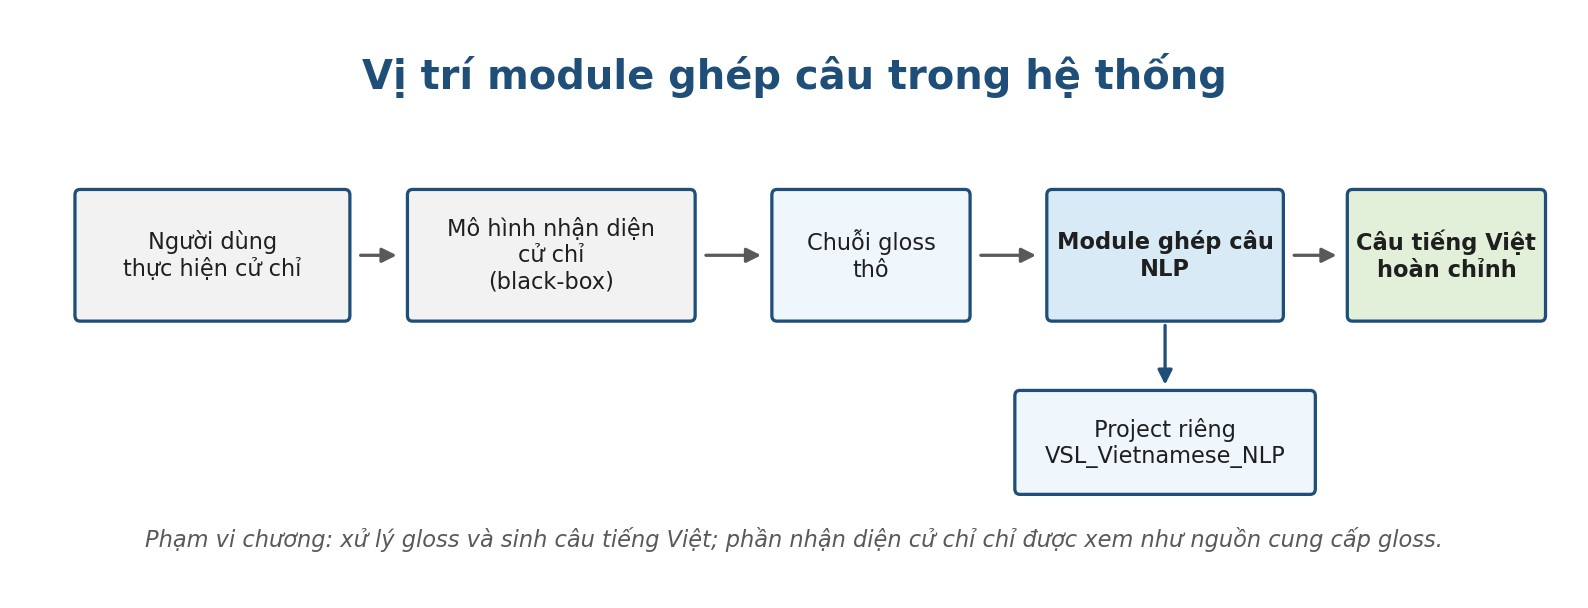
\includegraphics[width=0.95\textwidth]{figures/nlp/vsl_module_position.jpg}
\caption{Vị trí của mô-đun ghép câu trong hệ thống xử lý ký hiệu}
\label{fig:gloss-to-sentence-pipeline}
\end{figure}

\subsubsection{Phát biểu bài toán}

Cho một chuỗi gloss đầu vào nhận được từ tầng nhận diện ký hiệu, mô-đun ghép câu cần
sinh ra một chuỗi đầu ra là câu tiếng Việt hoàn chỉnh sao cho:
\begin{itemize}
    \item bảo toàn ý nghĩa cốt lõi của chuỗi gloss đầu vào;
    \item bổ sung được các thành phần ngữ pháp cần thiết cho tiếng Việt;
    \item giảm tính rời rạc, lặp từ và thiếu dấu câu của đầu ra trung gian;
    \item đủ nhẹ để tích hợp vào chế độ realtime.
\end{itemize}

Ví dụ, chuỗi \texttt{toi muon uong\_nuoc} không nên chỉ được hiển thị nguyên dạng, mà
cần được chuyển thành câu \textit{Tôi muốn uống nước.} Tương tự,
\texttt{toi can giup\_do} nên được chuyển thành \textit{Tôi cần giúp đỡ.}

\subsubsection{Kiến trúc lai được sử dụng}

Thay vì phụ thuộc hoàn toàn vào một mô hình sinh văn bản, project hiện thực mô-đun này
theo kiến trúc lai gồm ba tầng ưu tiên:
\begin{enumerate}
    \item \textbf{Rule-based/template}: tra cứu các mẫu câu có tần suất cao trong
    \codepath{configs/sentence_rules.json}. Đây là tầng có độ ổn định cao nhất và phản hồi
    rất nhanh.
    \item \textbf{BARTpho fine-tuned}: nếu chuỗi đầu vào không khớp rule cứng, hệ thống
    dùng mô hình sinh văn bản để phục hồi câu tiếng Việt linh hoạt hơn.
    \item \textbf{Fallback corrector}: nếu mô hình chưa được huấn luyện hoặc không thể
    nạp, hệ thống vẫn còn tầng dự phòng để ánh xạ token cơ bản và thêm dấu câu tối thiểu.
\end{enumerate}

Thiết kế này bám sát hiện thực trong mã nguồn: lớp \texttt{SentenceBuilder} lần lượt kiểm
tra rule, gọi predictor BARTpho và cuối cùng rơi về tầng fallback. Cách tổ chức như vậy giúp mô-đun vừa có khả năng sinh câu
tự nhiên, vừa đảm bảo tính an toàn khi triển khai thực tế.

\begin{figure}[H]
\centering
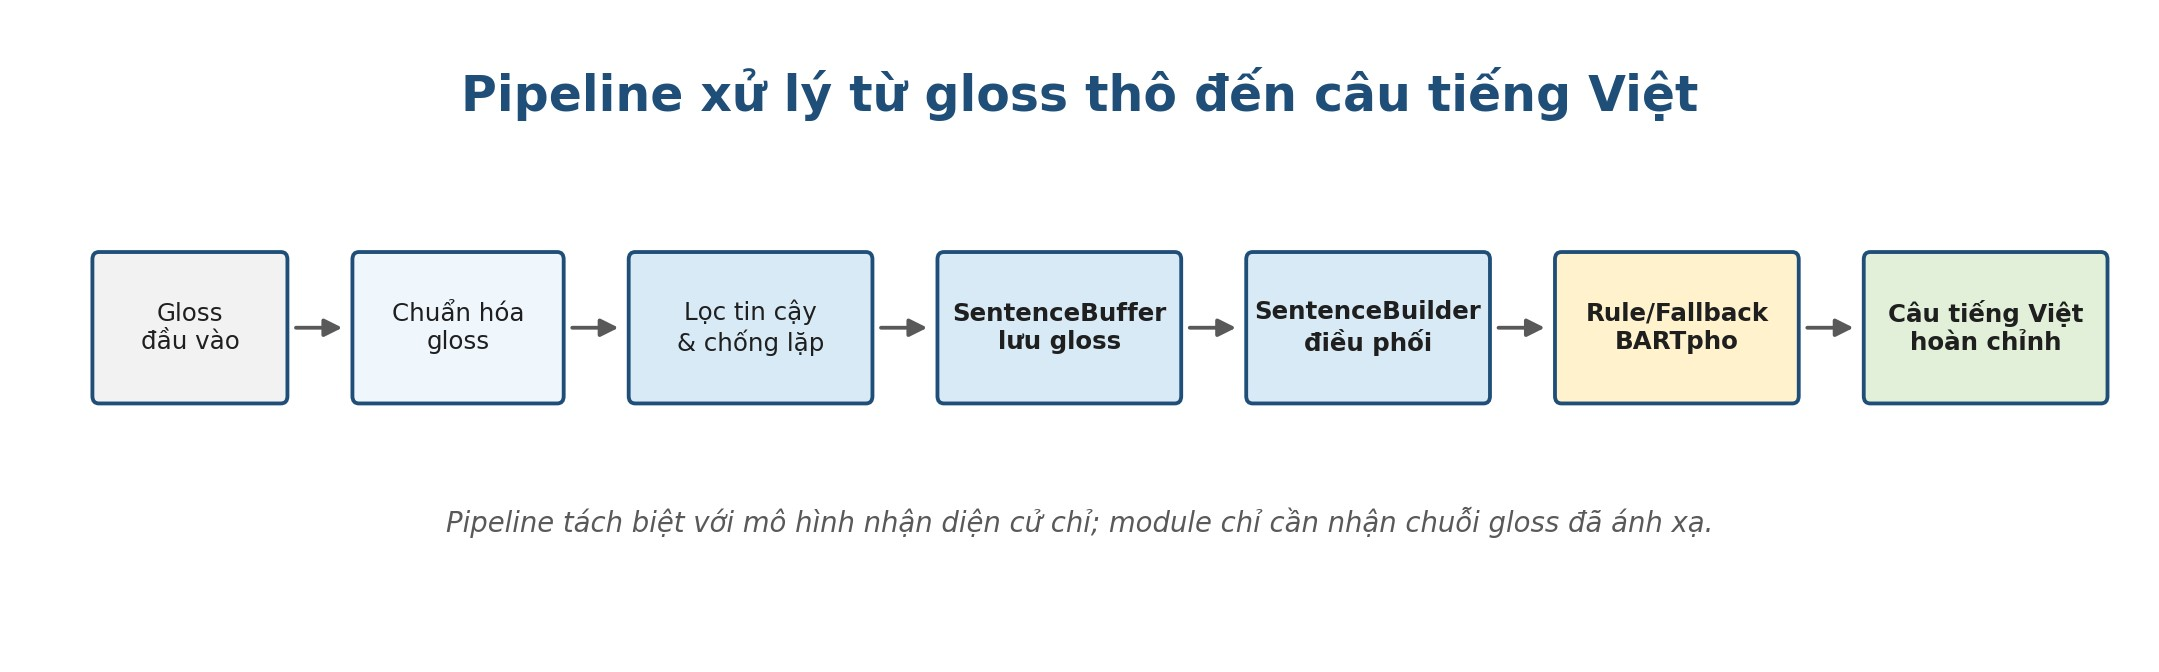
\includegraphics[width=0.95\textwidth]{figures/nlp/vsl_gloss_processing_pipeline.jpg}
\caption{Pipeline xử lý từ gloss thô đến câu tiếng Việt hoàn chỉnh}
\label{fig:vsl-gloss-processing-pipeline}
\end{figure}

\begin{figure}[H]
\centering
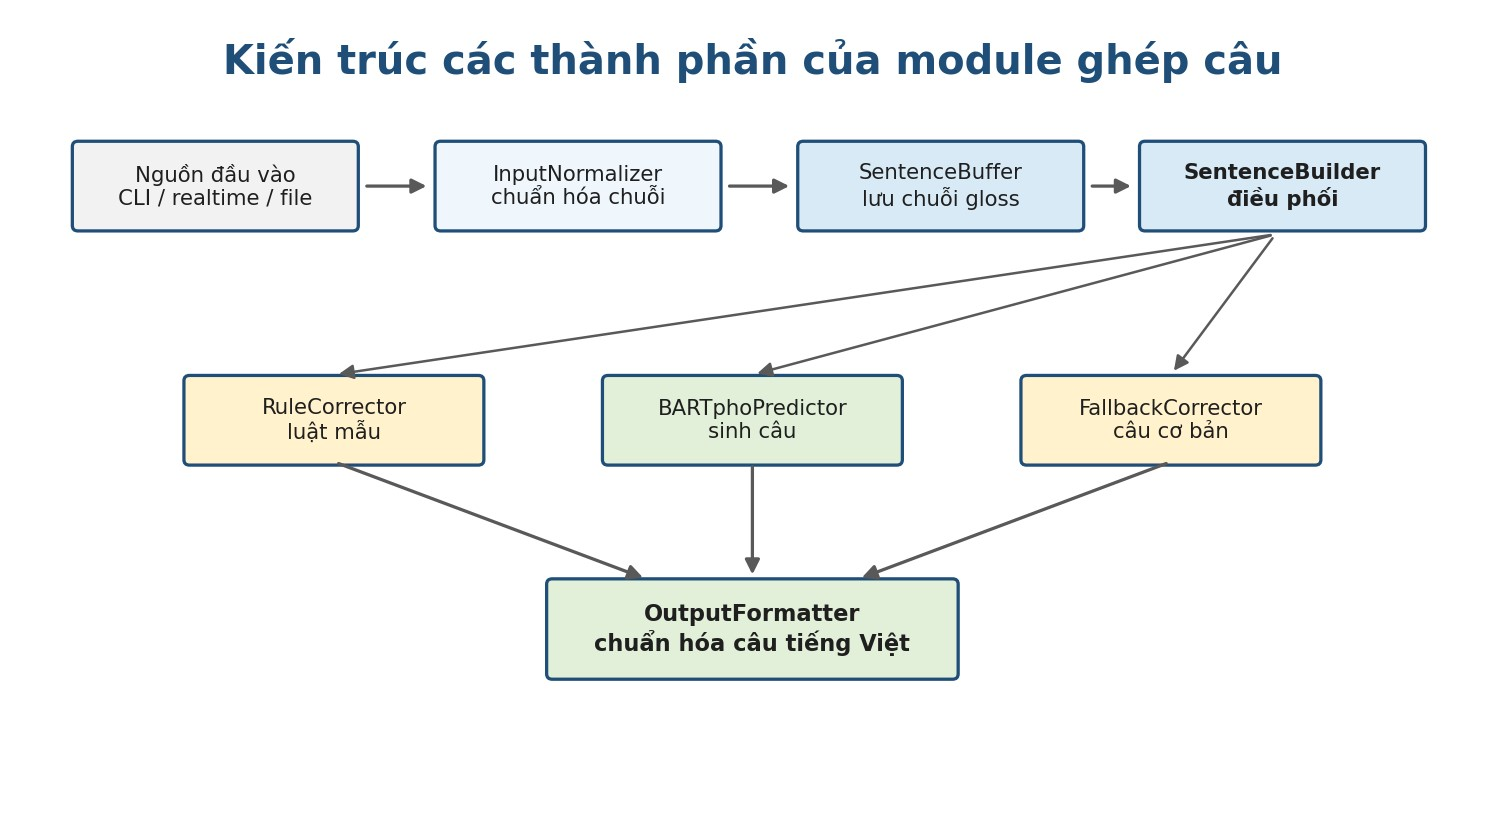
\includegraphics[width=0.9\textwidth]{figures/nlp/vsl_sentence_module_architecture.jpg}
\caption{Kiến trúc các thành phần chính của mô-đun ghép câu}
\label{fig:hybrid-sentence-builder}
\end{figure}

\begin{table}[H]
\centering
\caption{Vai trò của các thành phần trong mô-đun ghép câu}
\begin{tabularx}{\textwidth}{|p{3.2cm}|X|X|}
\hline
\textbf{Thành phần} & \textbf{Vai trò chính} & \textbf{Ý nghĩa trong hệ thống realtime} \\
\hline
Rule/template & Xử lý các mẫu giao tiếp ngắn, lặp lại nhiều lần như chào hỏi, xin lỗi, yêu cầu hỗ trợ. & Phản hồi gần như tức thời, giảm phụ thuộc vào mô hình sinh. \\
\hline
BARTpho fine-tuned & Khôi phục câu tự nhiên cho các chuỗi gloss linh hoạt hoặc chưa có rule. & Tăng độ tự nhiên và khả năng tổng quát hóa của đầu ra. \\
\hline
Fallback corrector & Ánh xạ token cơ bản, viết hoa đầu câu và thêm dấu câu tối thiểu. & Đảm bảo hệ thống vẫn sử dụng được khi mô hình chưa sẵn sàng. \\
\hline
\end{tabularx}
\end{table}

\subsubsection{Lý do chọn BARTpho}

BARTpho là mô hình \textit{sequence-to-sequence} đơn ngữ đầu tiên được tiền huấn luyện
quy mô lớn cho tiếng Việt. Theo Tran, Le và Nguyen, BARTpho có hai biến thể là
\textit{BARTpho-syllable} và \textit{BARTpho-word}; mô hình sử dụng kiến trúc
\textit{BART-large} và đặc biệt phù hợp với các tác vụ sinh văn bản tiếng Việt. Về gốc,
BART là một \textit{denoising autoencoder} kết hợp encoder hai chiều và decoder sinh
trái sang phải, nhờ đó rất phù hợp cho các tác vụ phục hồi câu, tóm tắt hoặc tái cấu trúc
chuỗi.

Trong project này, cấu hình \codepath{configs/nlp_config.json} chọn mô hình nền BARTpho word-base. Đây là lựa chọn hợp lý vì:
\begin{itemize}
    \item đầu vào của mô-đun đã ở dạng token từ hoặc cụm từ phân cách bằng khoảng
    trắng;
    \item nhiều gloss dùng dấu gạch dưới để biểu diễn cụm từ cố định như
    \texttt{uong\_nuoc}, \texttt{benh\_vien}, \texttt{giup\_do};
    \item mô hình đơn ngữ tiếng Việt thường diễn đạt câu đích mượt hơn so với mô hình đa
    ngôn ngữ tổng quát khi tác vụ chỉ có một ngôn ngữ đầu ra.
\end{itemize}

Để đồng nhất giữa huấn luyện và suy luận, project thêm tiền tố nhiệm vụ \codepath{chuyen_cau_ky_hieu:}
vào chuỗi đầu vào trước khi token hóa. Đây là một chi tiết
quan trọng vì giúp mô hình hiểu đúng ngữ cảnh nhiệm vụ sinh câu, đồng thời tránh lệch
phân phối giữa train và inference.

\begin{figure}[H]
\centering
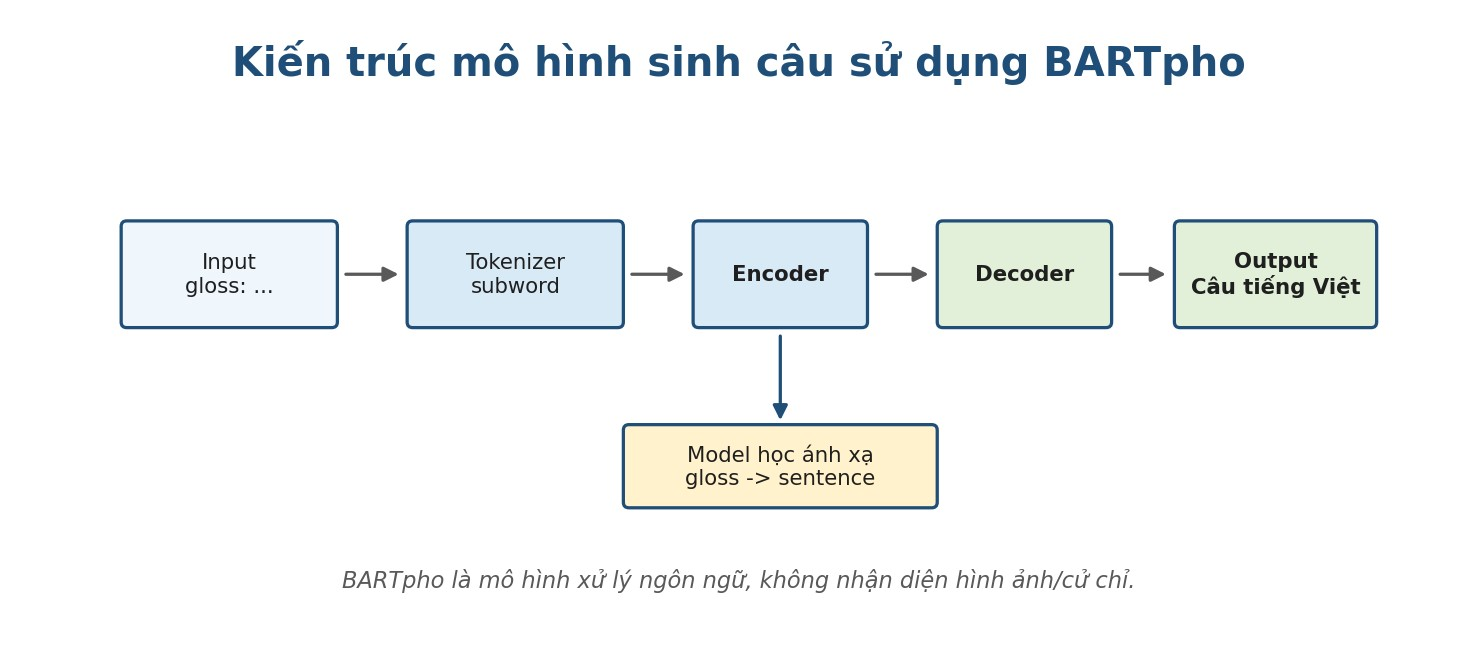
\includegraphics[width=0.88\textwidth]{figures/nlp/vsl_bartpho_generation_architecture.jpg}
\caption{Kiến trúc sinh câu tiếng Việt bằng BARTpho}
\label{fig:bartpho-architecture}
\end{figure}

\subsubsection{Thông số thiết kế chính}

Các thông số nổi bật đang được dùng trong project gồm:
\begin{itemize}
    \item mô hình nền: \texttt{vinai/bartpho-word-base};
    \item độ dài tối đa đầu vào: 64 token;
    \item độ dài tối đa đầu ra: 64 token;
    \item huấn luyện với \texttt{AdamW}, learning rate \texttt{5e-5};
    \item suy luận dùng \texttt{beam search} với \texttt{num\_beams = 4}.
\end{itemize}

Bên cạnh cấu hình suy luận/demo đang lưu trong repository, tài liệu \texttt{vsl.pdf} ghi nhận
lần fine-tune chính của BARTpho được thực hiện trên Google Colab với cấu hình dài hơn cho
chuỗi nguồn và chuỗi đích. Cấu hình này được dùng làm căn cứ cho phần đánh giá ở
Chương~4.

\begin{table}[H]
\centering
\caption{Cấu hình fine-tune BARTpho}
\label{tab:bartpho-finetune-config-vsl}
\begin{tabularx}{0.86\textwidth}{|X|c|}
\hline
\textbf{Thành phần} & \textbf{Giá trị} \\
\hline
Môi trường & Google Colab \\
\hline
GPU & T4 \\
\hline
Mô hình gốc & BARTpho \\
\hline
Số epoch & 5 \\
\hline
Batch size & 4 \\
\hline
Max source length & 96 \\
\hline
Max target length & 128 \\
\hline
\end{tabularx}
\end{table}

\begin{figure}[H]
\centering
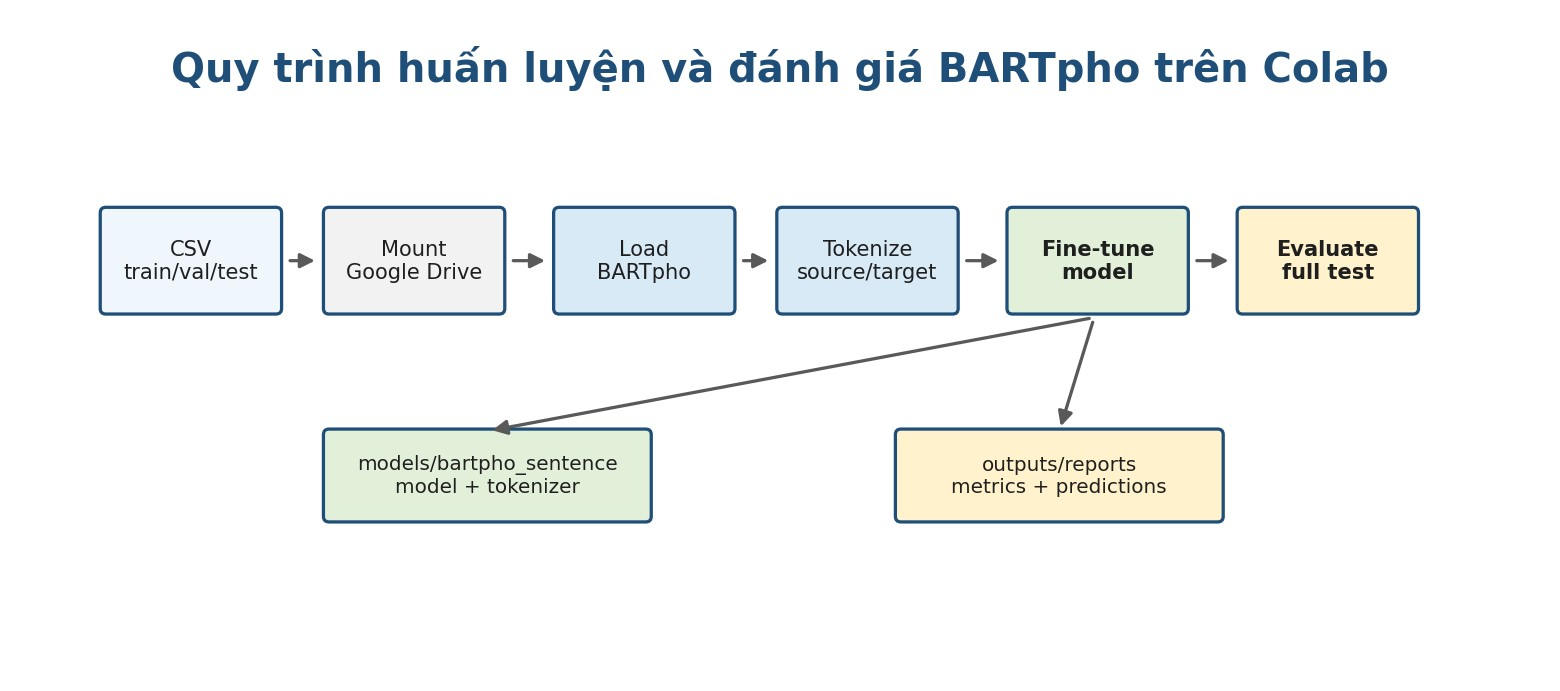
\includegraphics[width=0.9\textwidth]{figures/nlp/vsl_bartpho_training_evaluation_pipeline.jpg}
\caption{Quy trình huấn luyện và đánh giá BARTpho}
\label{fig:vsl-bartpho-training-evaluation-pipeline}
\end{figure}

Tập luật hiện tại đóng vai trò như một lớp tri thức miền hẹp, đặc biệt hữu ích với các câu
giao tiếp chăm sóc sức khỏe hoặc nhu cầu cơ bản. Khi gloss đầu vào chưa có trong tập
luật, BARTpho đảm nhiệm phần tổng quát hóa. Nếu cả hai đường này đều không khả dụng,
fallback sẽ duy trì đầu ra đọc được thay vì làm hỏng toàn bộ pipeline.

\subsubsection{Ưu điểm và giới hạn}

Ưu điểm lớn nhất của kiến trúc hiện tại là cân bằng giữa \textit{độ ổn định} và
\textit{độ tự nhiên}. Rule-based giúp giữ đúng các mẫu câu quan trọng, còn BARTpho cho
phép mô-đun không bị giới hạn ở một tập câu cứng. Điều này đặc biệt phù hợp với hệ
thống thời gian thực, nơi lỗi của tầng nhận diện trước đó có thể lan sang tầng NLP.

Tuy nhiên, mô-đun này vẫn có một số giới hạn:
\begin{itemize}
    \item nếu chuỗi gloss đầu vào sai quá nhiều do nhận diện nhầm, mô hình sinh câu vẫn có
    thể bảo toàn lỗi ngữ nghĩa;
    \item tập luật hiện tại phù hợp nhất với miền giao tiếp cơ bản, chưa đủ bao phủ hội thoại
    mở;
    \item chất lượng metric rất cao trên bộ dữ liệu sinh theo template không đồng nghĩa với
    khả năng tổng quát hóa hoàn toàn ngoài miền dữ liệu đó.
\end{itemize}

